
\begin{block}{\color{mydarkgreen}{Experiment Results}}


% \textbf{Datasets}: CoQA (coqa), TriviaQA (trivia), Natural Questions (nq)

% \textbf{Models}:  LLaMA (13B), LLaMA2 (13B), OPT (13B), gpt-3.5-turbo

\textbf{Evaluation Metrics}: 
\begin{itemize}
    \item AUARC: Area under the Accuracy-Rejection Curve. 
    The curve computes the accuracy at each rejection threshold (low-confidence responses or high-uncertainty questions are rejected).
    \item AUROC: $\mathbf{1}\{{\mathbf{s}\text{ correctly answers } \mathbf{x}}\}\sim$ $C(\mathbf{x}, \mathbf{s})$ or $-U(\mathbf{x})$.
\end{itemize}


\begin{figure}[htbp]
  \centering
  \begin{minipage}[b]{0.99\textwidth}
    \centering
    \resizebox{\textwidth}{!}{%
      \begin{tabular}{lc|cccc|cccc|cccc}
\toprule
  &   & trivia(llama) & trivia(llama2) & trivia(opt) & trivia(gpt) & coqa(llama) & coqa(llama2) & coqa(opt) & coqa(gpt) & nq(llama) & nq(llama2) & nq(opt) & nq(gpt)\\
\midrule
\multirow{2}{*}{} & Random & 61.18$\pm$0.07 & 76.24$\pm$0.11 & 25.75$\pm$0.12 & 87.42$\pm$0.08 & 62.46$\pm$0.11 & 78.71$\pm$0.13 & 53.81$\pm$0.18 & 79.76$\pm$0.14 & 23.63$\pm$0.36 & 44.13$\pm$0.68 & 8.60$\pm$0.18 & 62.72$\pm$0.39\\
  & Oracle & 87.03$\pm$0.05 & 96.50$\pm$0.03 & 54.72$\pm$0.19 & 99.09$\pm$0.01 & 86.29$\pm$0.06 & 96.92$\pm$0.03 & 79.41$\pm$0.14 & 97.45$\pm$0.03 & 47.67$\pm$0.55 & 77.62$\pm$0.63 & 23.28$\pm$0.43 & 90.65$\pm$0.21\\
\midrule
\multirow{2}{*}{Baselines} & \baselineNumSets & 78.78$\pm$0.17 & 91.37$\pm$0.12 & 39.46$\pm$0.29 & 93.18$\pm$0.11 & 67.58$\pm$0.17 & 83.66$\pm$0.17 & 60.41$\pm$0.27 & 80.69$\pm$0.22 & 28.18$\pm$0.55 & 57.55$\pm$0.98 & 10.36$\pm$0.27 & 68.92$\pm$0.74\\
  & \baselineLexiSim & 80.32$\pm$0.06 & 91.73$\pm$0.13 & 45.68$\pm$0.24 & 94.69$\pm$0.15 & 78.17$\pm$0.15 & 89.29$\pm$0.16 & 71.46$\pm$0.21 & 86.60$\pm$0.13 & 40.15$\pm$0.70 & 61.88$\pm$1.14 & 15.92$\pm$0.55 & 73.40$\pm$0.74\\
\midrule
\multirow{3}{*}{Ours} & \methodEigvClip(E) & 85.01$\pm$0.08 & \textbf{93.07$\pm$0.17} & 51.54$\pm$0.21 & \underline{\textbf{95.16$\pm$0.21}} & 81.27$\pm$0.12 & \underline{\textbf{90.21$\pm$0.24}} & 73.46$\pm$0.20 & \underline{\textbf{88.80$\pm$0.10}} & \underline{\textbf{40.42$\pm$0.67}} & \underline{\textbf{63.58$\pm$0.96}} & 18.20$\pm$0.44 & \underline{\textbf{75.17$\pm$0.80}}\\
  & \methodEcc(E) & 84.66$\pm$0.06 & \textbf{93.12$\pm$0.12} & 51.42$\pm$0.22 & \underline{\textbf{95.21$\pm$0.22}} & 80.55$\pm$0.14 & \underline{\textbf{90.02$\pm$0.22}} & 72.73$\pm$0.20 & 88.67$\pm$0.13 & 40.38$\pm$0.68 & \underline{\textbf{63.41$\pm$0.92}} & \underline{\textbf{18.82$\pm$0.46}} & \underline{\textbf{75.40$\pm$0.49}}\\
  & \methodDegree(E) & \underline{\textbf{85.27$\pm$0.06}} & \textbf{93.05$\pm$0.14} & \underline{\textbf{52.06$\pm$0.21}} & \underline{\textbf{95.00$\pm$0.23}} & \underline{\textbf{81.50$\pm$0.15}} & \underline{\textbf{90.18$\pm$0.22}} & \underline{\textbf{73.91$\pm$0.19}} & 88.63$\pm$0.23 & \underline{\textbf{41.07$\pm$0.69}} & \underline{\textbf{63.41$\pm$1.03}} & \underline{\textbf{18.43$\pm$0.48}} & 74.35$\pm$0.78\\
\midrule
\multirow{2}{*}{White-box} & \baselineGal & 79.15$\pm$0.08 & \underline{93.99$\pm$0.06} & 51.11$\pm$0.20 & \textendash & 78.83$\pm$0.16 & 89.29$\pm$0.17 & 70.75$\pm$0.21 & \textendash & 36.03$\pm$0.54 & 62.40$\pm$0.98 & \underline{18.40$\pm$0.44} & \textendash\\
  & \baselinePTrue & 64.98$\pm$0.10 & 82.53$\pm$0.09 & 20.25$\pm$0.11 & \textendash & 64.04$\pm$0.18 & 79.92$\pm$0.17 & 50.23$\pm$0.23 & \textendash & 24.72$\pm$0.42 & 44.25$\pm$0.65 & 7.63$\pm$0.22 & \textendash\\
\bottomrule
\bottomrule
\end{tabular}
    }
    \captionof{table}{
    AUARC when using $U(x)$ to predict expected accuracy.
The best black-box methods are in \textbf{bold} and the best overall is \underline{underscored}.
In general, our proposed uncertainty measures perform significantly better than the baselines, sometimes outperforming the white-box methods.
    }
    \label{table:main:exp:arc:u+ea}
  \end{minipage}
\end{figure}


\begin{figure}[htbp]
  \centering
  \begin{minipage}[b]{0.99\textwidth}
    \centering
    \resizebox{\textwidth}{!}{%
      \begin{tabular}{lc|cccc|cccc|cccc}
\toprule
  %& \multicolumn{4}{c}{Baselines}& \multicolumn{9}{|c|}{Ours}& \multicolumn{2}{c}{White-box}\\
    &   & trivia(llama) & trivia(llama2) & trivia(opt) & trivia(gpt) & coqa(llama) & coqa(llama2) & coqa(opt) & coqa(gpt) & nq(llama) & nq(llama2) & nq(opt) & nq(gpt)\\
\midrule
\multirow{2}{*}{} & Random & 61.18$\pm$0.07 & 76.24$\pm$0.11 & 25.75$\pm$0.12 & 87.42$\pm$0.08 & 62.46$\pm$0.11 & 78.71$\pm$0.13 & 53.81$\pm$0.18 & 79.76$\pm$0.14 & 23.63$\pm$0.36 & 44.13$\pm$0.68 & 8.60$\pm$0.18 & 62.72$\pm$0.39\\
  & Oracle & 91.24$\pm$0.03 & 96.92$\pm$0.03 & 60.68$\pm$0.16 & 99.17$\pm$0.01 & 91.85$\pm$0.05 & 97.55$\pm$0.03 & 87.15$\pm$0.11 & 97.80$\pm$0.03 & 57.69$\pm$0.53 & 80.22$\pm$0.56 & 29.65$\pm$0.45 & 91.97$\pm$0.18\\
\midrule
\multirow{2}{*}{Baselines} & \baselineNumSets & 78.78$\pm$0.17 & 91.37$\pm$0.12 & 39.46$\pm$0.29 & 93.18$\pm$0.11 & 67.58$\pm$0.17 & 83.66$\pm$0.17 & 60.41$\pm$0.27 & 80.69$\pm$0.22 & 28.18$\pm$0.55 & 57.55$\pm$0.98 & 10.36$\pm$0.27 & 68.92$\pm$0.74\\
  & \baselineLexiSim & 80.32$\pm$0.06 & 91.73$\pm$0.13 & 45.68$\pm$0.24 & 94.69$\pm$0.15 & 78.17$\pm$0.15 & 89.29$\pm$0.16 & 71.46$\pm$0.21 & 86.60$\pm$0.13 & 40.15$\pm$0.70 & 61.88$\pm$1.14 & 15.92$\pm$0.55 & 73.40$\pm$0.74\\
\midrule
\multirow{3}{*}{Ours} & \methodEigvClip(E) & 85.01$\pm$0.08 & 93.07$\pm$0.17 & 51.54$\pm$0.21 & \underline{\textbf{95.16$\pm$0.21}} & 81.27$\pm$0.12 & \underline{\textbf{90.21$\pm$0.24}} & 73.46$\pm$0.20 & \underline{\textbf{88.80$\pm$0.10}} & 40.42$\pm$0.67 & \underline{\textbf{63.58$\pm$0.96}} & 18.20$\pm$0.44 & \underline{\textbf{75.17$\pm$0.80}}\\
  & \methodEcc(E) & 88.17$\pm$0.11 & \textbf{93.21$\pm$0.07} & 55.82$\pm$0.21 & \underline{\textbf{95.11$\pm$0.18}} & \underline{\textbf{84.62$\pm$0.13}} & \underline{\textbf{90.21$\pm$0.25}} & \underline{\textbf{78.14$\pm$0.20}} & 88.42$\pm$0.19 & 45.78$\pm$0.69 & \underline{\textbf{63.89$\pm$1.08}} & \underline{\textbf{21.00$\pm$0.49}} & \underline{\textbf{75.43$\pm$0.67}}\\
  & \methodDegree(E) & \underline{\textbf{88.86$\pm$0.05}} & \textbf{93.19$\pm$0.11} & \underline{\textbf{56.11$\pm$0.19}} & 94.94$\pm$0.16 & \underline{\textbf{84.60$\pm$0.15}} & 89.75$\pm$0.19 & 77.83$\pm$0.20 & 88.02$\pm$0.31 & \underline{\textbf{46.54$\pm$0.69}} & \underline{\textbf{63.55$\pm$1.01}} & \underline{\textbf{21.30$\pm$0.50}} & 74.67$\pm$0.64\\
\midrule
\multirow{2}{*}{White-box} & \baselineGal & 79.15$\pm$0.08 & \underline{93.99$\pm$0.06} & 51.11$\pm$0.20 & \textendash & 78.83$\pm$0.16 & 89.29$\pm$0.17 & 70.75$\pm$0.21 & \textendash & 36.03$\pm$0.54 & 62.40$\pm$0.98 & 18.40$\pm$0.44 & \textendash\\
  & \baselinePTrue & 67.27$\pm$0.11 & 82.18$\pm$0.08 & 20.89$\pm$0.12 & \textendash & 66.23$\pm$0.19 & 79.55$\pm$0.16 & 49.84$\pm$0.23 & \textendash & 27.62$\pm$0.46 & 44.34$\pm$0.64 & 8.07$\pm$0.21 & \textendash\\
\bottomrule
\end{tabular}
    }
\captionof{table}{
AUARC when using $C(x,\mathbf{s})$ to predict individual accuracy.
AUARC generally improves compared with Table 1.
% The best black-box methods are in \textbf{bold} and the best overall is \underline{underscored}.
% Compared with~\cref{table:main:exp:arc:u+ea}, the AUARC for confidence measures (\methodDegree and \methodEcc) generally improve, as they could discriminate the quality of each response. 
}
\label{table:main:exp:arc:c+ia}
  \end{minipage}
\end{figure}


\begin{figure}[ht]
    \centering
    %\vspace{-3mm}%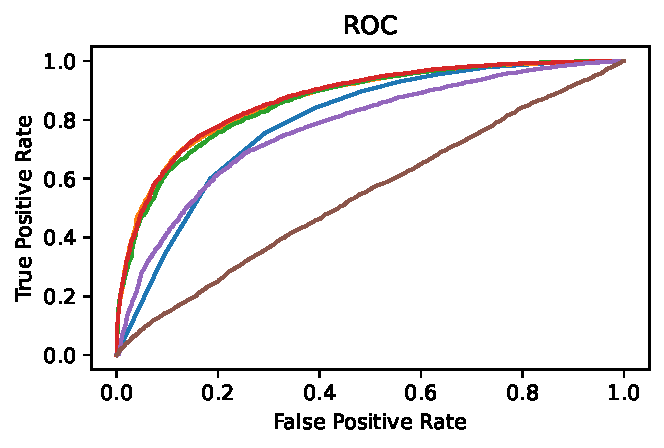
\includegraphics[width=0.45\textwidth]{pics/trivia_llama_auroc.pdf}%
    %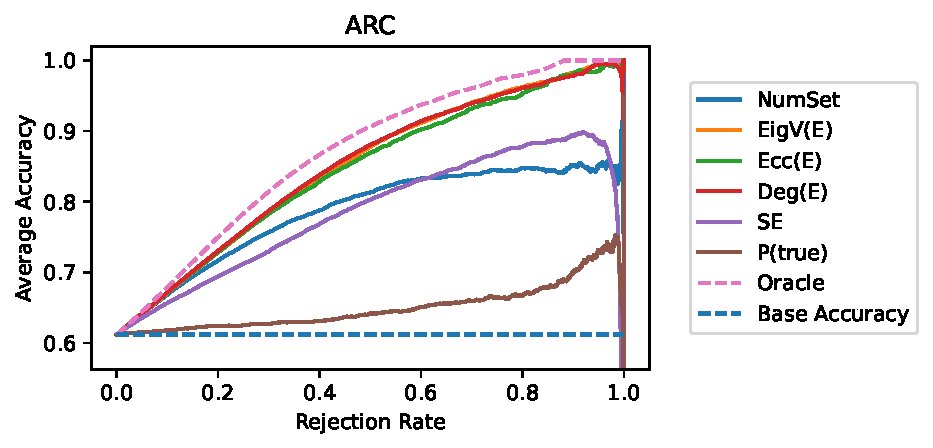
\includegraphics[width=0.45\textwidth]{pics/trivia_llama_auarc.pdf}
    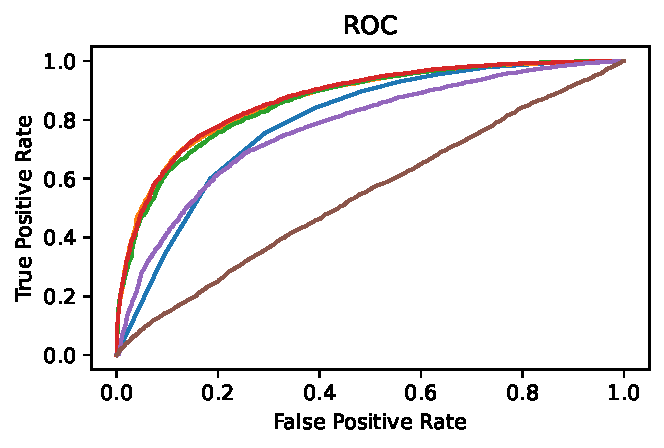
\includegraphics[height=10cm]{pics/trivia_llama_auroc.pdf}%
    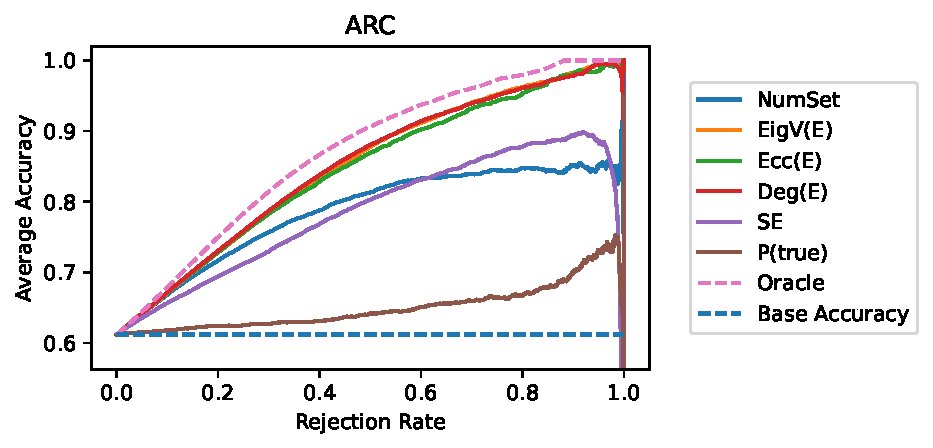
\includegraphics[height=10cm]{pics/trivia_llama_auarc.pdf}
    \caption{The ROC (left) computed using the accuracy of the 1st generated response and the corresponding confidence $C$ (when available, otherwise $U$), for LLaMA on \datasettrivia.
    ARC (right) is computed using $U$ and expected accuracy. 
    % (For ARC, average accuracy is noisy at high rejection rate due to small sample size.) 
    The suffix (E) denotes for $a_{NLI,entail}$. 
    % Different ways to construct $U$ or $C$ from $a_{NLI,entail}$ make a relatively small difference, but are all noticeably better than the baselines (including the white-box baselines).
    % The ARC suggests that if we select only the top 50\% samples using, for example, \methodDegree(E), we could improve the accuracy from 62\% to around 90\%. 
    }
    \label{fig:auroc_auarc}
\end{figure}

\end{block}

%----------------------------------------------------------------------------------------
%	REFERENCES
%----------------------------------------------------------------------------------------

%\begin{block}{References}

%\nocite{*} % Insert publications even if they are not cited in the poster
%\small{\bibliographystyle{unsrt}
%\bibliography{new_poster}\vspace{0.75in}}

%\end{block}

%----------------------------------------------------------------------------------------
%	ACKNOWLEDGEMENTS
%----------------------------------------------------------------------------------------

\setbeamercolor{block title}{fg=red,bg=white} % Change the block title color

\begin{block}{Acknowledgements}

\small{\rmfamily{This work was supported by NSF award SCH-2205289, SCH-2014438, IIS-1838042, NIH award R01 1R01NS107291-01.}} \\

\end{block}

%----------------------------------------------------------------------------------------
%	CONTACT INFORMATION
%----------------------------------------------------------------------------------------

\setbeamercolor{block alerted title}{fg=black,bg=norange} % Change the alert block title colors
\setbeamercolor{block alerted body}{fg=black,bg=white} % Change the alert block body colors

\begin{alertblock}{Additional Information}

\begin{itemize}
\item Code: \href{https://github.com/zlin7/UQ-NLG}{https://github.com/zlin7/UQ-NLG}
\item Email: \href{mailto:zhenlin4@illinois.edu}{zhenlin4@illinois.edu}
\end{itemize}

\end{alertblock}